\chapter{Field Studies}
\section*{Purpose}
The purpose of the studies was to understand how nurses and surgeons train to operate a da Vinci robot and perform robot assisted minimal invasive surgery (RAMIS), as well as to asses what must be included in a surgery scenario.

\section*{Method}
We observed training sessions and a real surgery at Minimally Invasive Education Centre (MIUC) followed by a semi-structured interviews with Jane Petersson, First Nurse Assistant and Nurse Specialist in Robot Surgery, and Johan Poulsen, Head Surgeon at Aalborg Univeristy Hospital, to get an understanding of RAMIS and how surgeons practise. We conduct a contextual inquiry, which requires observations of the context, in this case both the training room and operating room, and the interviews with the two experts provide information about important procedures and tools. They also clarify observations, in case of ambiguity. 

The observation team took both pictures, notes, and recording video from the operation. Notes from this study are found in \autoref{ch:surgery_obs}. These illustrate the tasks and teamwork necessary to perform such an operation and were used to create different models; a physical model showing the layout of the room, a sequence model to clarify the work flow, and an artefact model showing objects used during the procedure.

\section*{Results}
The results are split into three sections; surgeon training at MIUC, team training focused interview at MIUC, surgery observation.

\subsection*{Surgeon Training at MIUC}
The training sessions at MIUC varies depending on the skill level of the participants. In cases with skilled participants, the students take on the role as instructors to help guide during the training session. This is beneficial as the surgeon often will be in charge during surgery.

During the interview, Jane Petersson explained that during team training a surgeon will operate the robot while making calls for the nurses in training. The individual tasks for the nurses depend on their current role. For instance, a first assistant nurse is the one who assists the surgeon inside of the patient. In general, the training focuses highly on getting familiar with the robot and how it operates during surgery. One particular task is important for the nurses to learn - how to dock the robot. As stated by both Jane Petersson and Johan Poulsen, ensuring that the robot is correctly docked is key to enable full movability of the robot. Johan Poulsen also expressed the importance of sterility of staff and tools.

\subsection*{Team Training Focused Interview at MIUC}
One of the most important things during surgery and training is the emergency handling, however this requires extensive knowledge of the robot and tools. Another very important task is the placement of the robot arms because collisions during surgery can be very dangerous. Sometimes the surgeons adjust the arms manually. In general, the training is for hands on experience with the robot and individual instruments, in preparation for a real surgery.

Teams during surgery, from which roles during team training are practised, consist of:
\begin{itemize}
  \item First assistant nurse - Sterile, assists the surgeon inside the patient's body.
  \item Scrub nurse - Sterile, prepare unpacked tools for the first assistant nurse.
  \item Circulating nurse - Not sterile, unpacks tools, and can go outside the sterile area.
\end{itemize}  

During training, on the first day Jane Petersson starts by introducing the robot and showing how tasks are done, while students observe. They also get hands-on experience with docking and moving the robot arms. On the second day, students are expected to do most of the tasks themselves. At the end of the second day, Jane Petersson sabotages some of the equipment and the students have to find and fix the errors. Any mistakes done by the students are used for learning purposes. At the beginning of the training, Jane Petersson makes most of the decisions, however later the students are expected to take the lead.

\subsection*{Surgery Observation}
The physical model shows the layout of the operation room and the staff's workspace. The figure includes doors and their movement as well as other objects. The layout is shown in \autoref{fig:layout}.

\begin{figure}[hpbt]
	\centering
	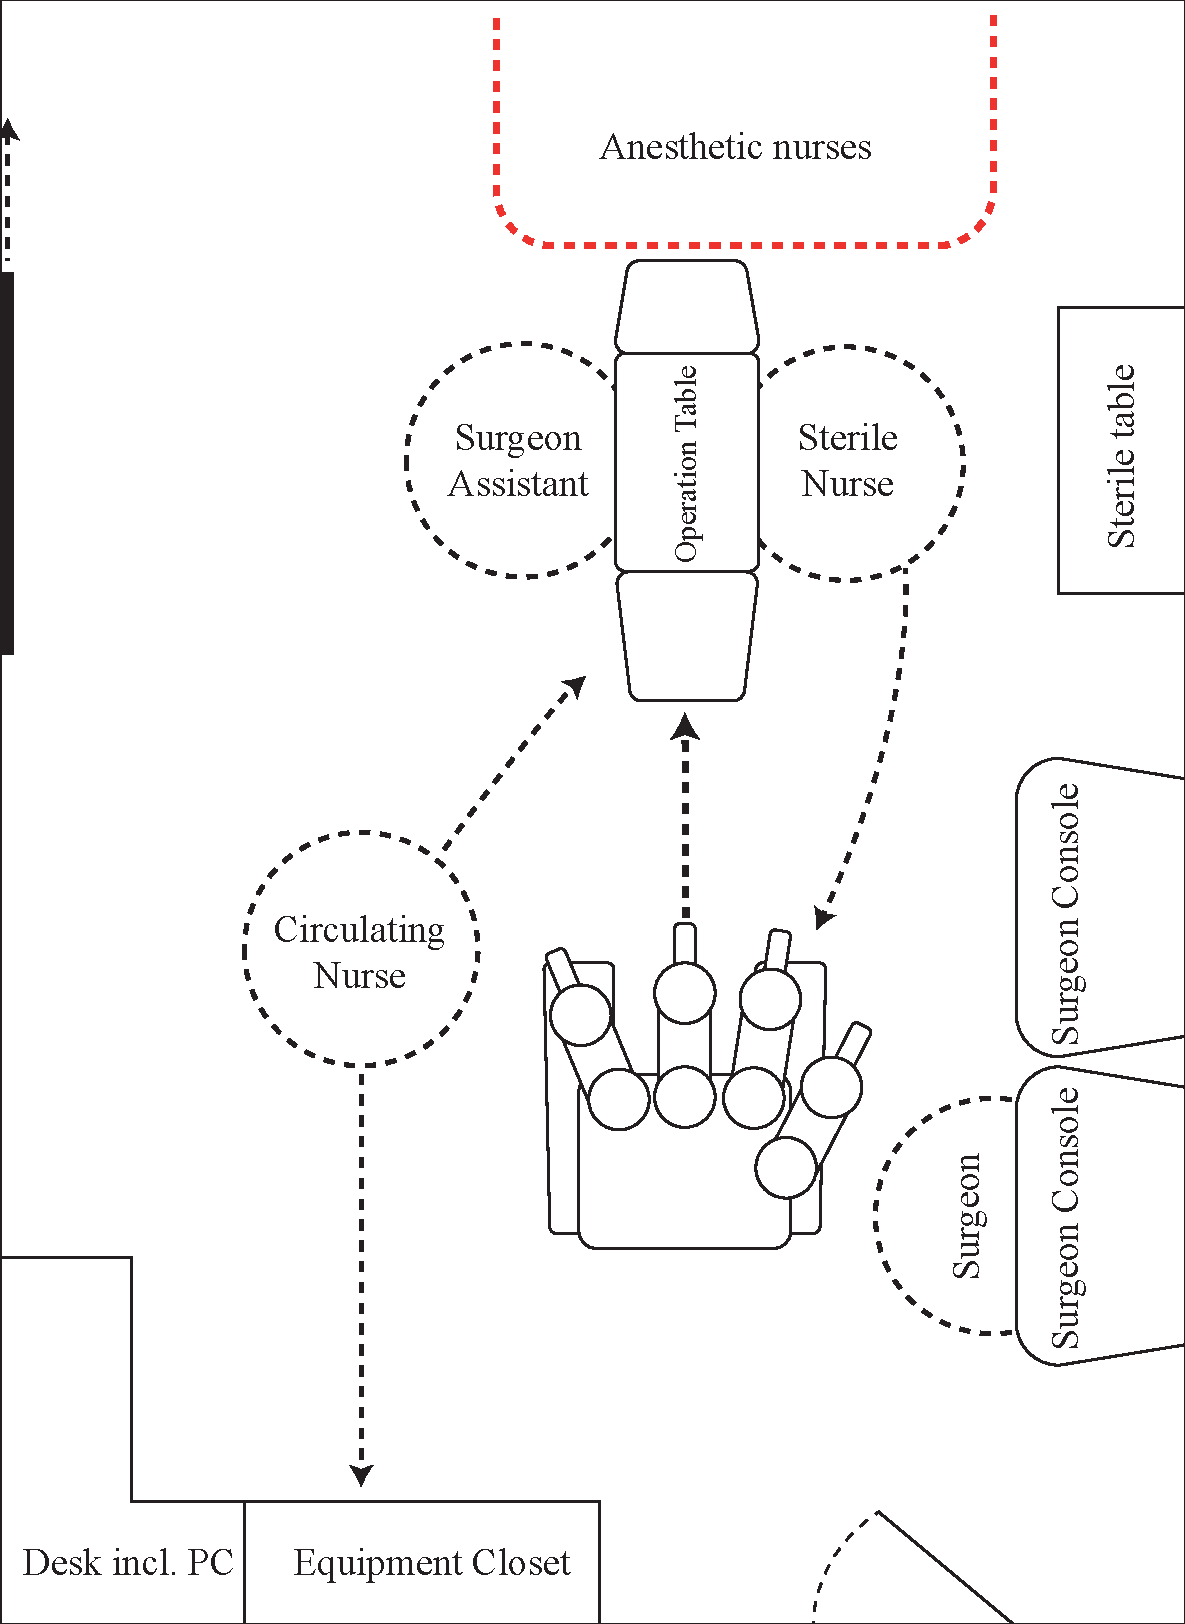
\includegraphics[width=0.5\textwidth]{FieldStudies/figures/physical}
	\caption{The phyiscal model showing the layout of the operation room}
	\label{fig:layout}
\end{figure}

The physical model enables the development and design of the room when creating the simulation.

The sequence model is based on Jane Petersson's worksheet used in team training at MUIC. The sequence model is shown in \autoref{fig:sequence}.

\begin{figure}[hbpt]
	\centering
	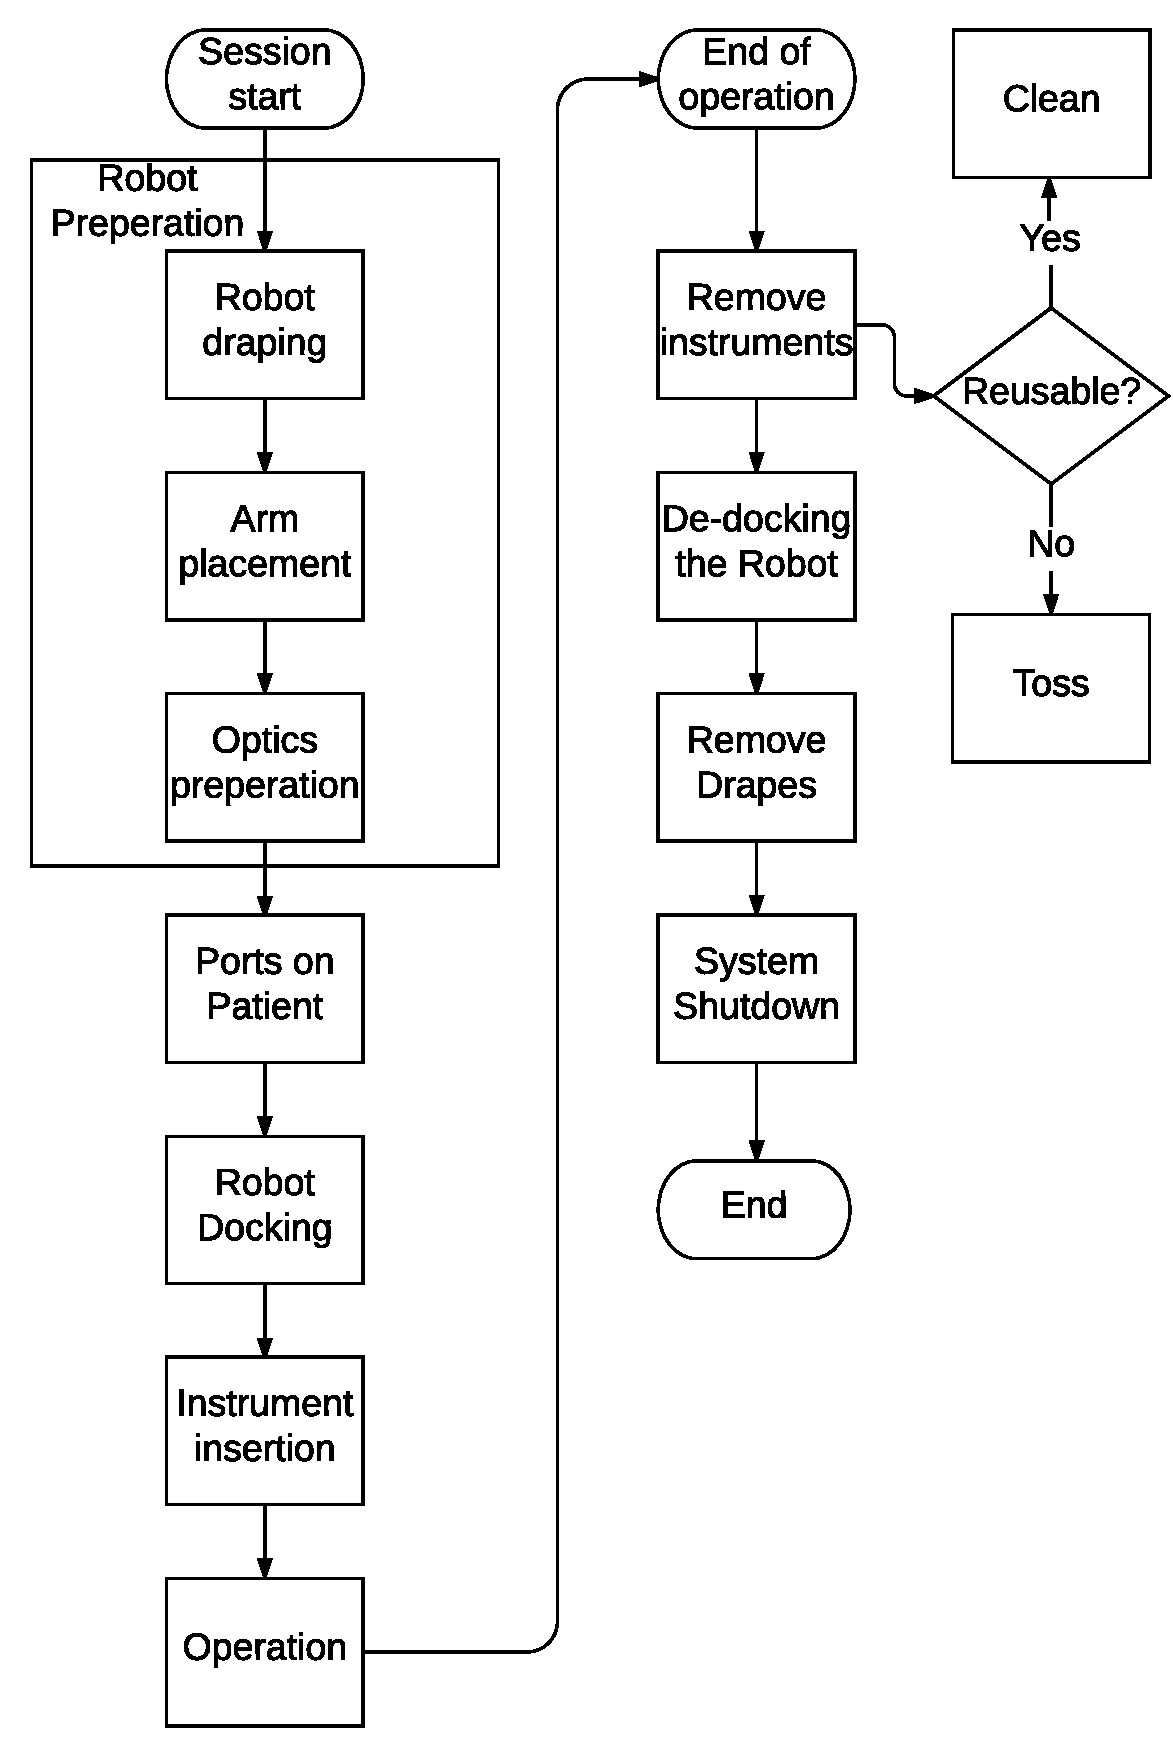
\includegraphics[width=0.75\textwidth]{FieldStudies/figures/sequencemodel}
	\caption{Flowchart of the sequence model showing how the operation preparation and debrief is carried out}
	\label{fig:sequence}
\end{figure}

The sequence model describes the actions necessary to both start the operation and to end it. This enables the design of the tasks which should be included in the simulation and their order of appearance to the user.
The model shown is for an operation without any complications. Complications can lead to undocking the robot in an emergency.


The Artefact models are shown in Figures \ref{fig:drapes}, \ref{fig:camera}, \ref{fig:cam_close}, \ref{fig:port}, and \ref{fig:tools}. These are created from pictures taken during the observation. \autoref{fig:drapes} shows the plastic drapes used to cover the arms of the robot sterilising it. \autoref{fig:camera} shows the endoscopic camera during calibration. \autoref{fig:cam_close} shows the endoscopic camera up close. \autoref{fig:port} shows one of the ports used to insert the tools into the patient. \autoref{fig:tools} shows the tools used with the robot.


\begin{figure}[H]
	\centering
	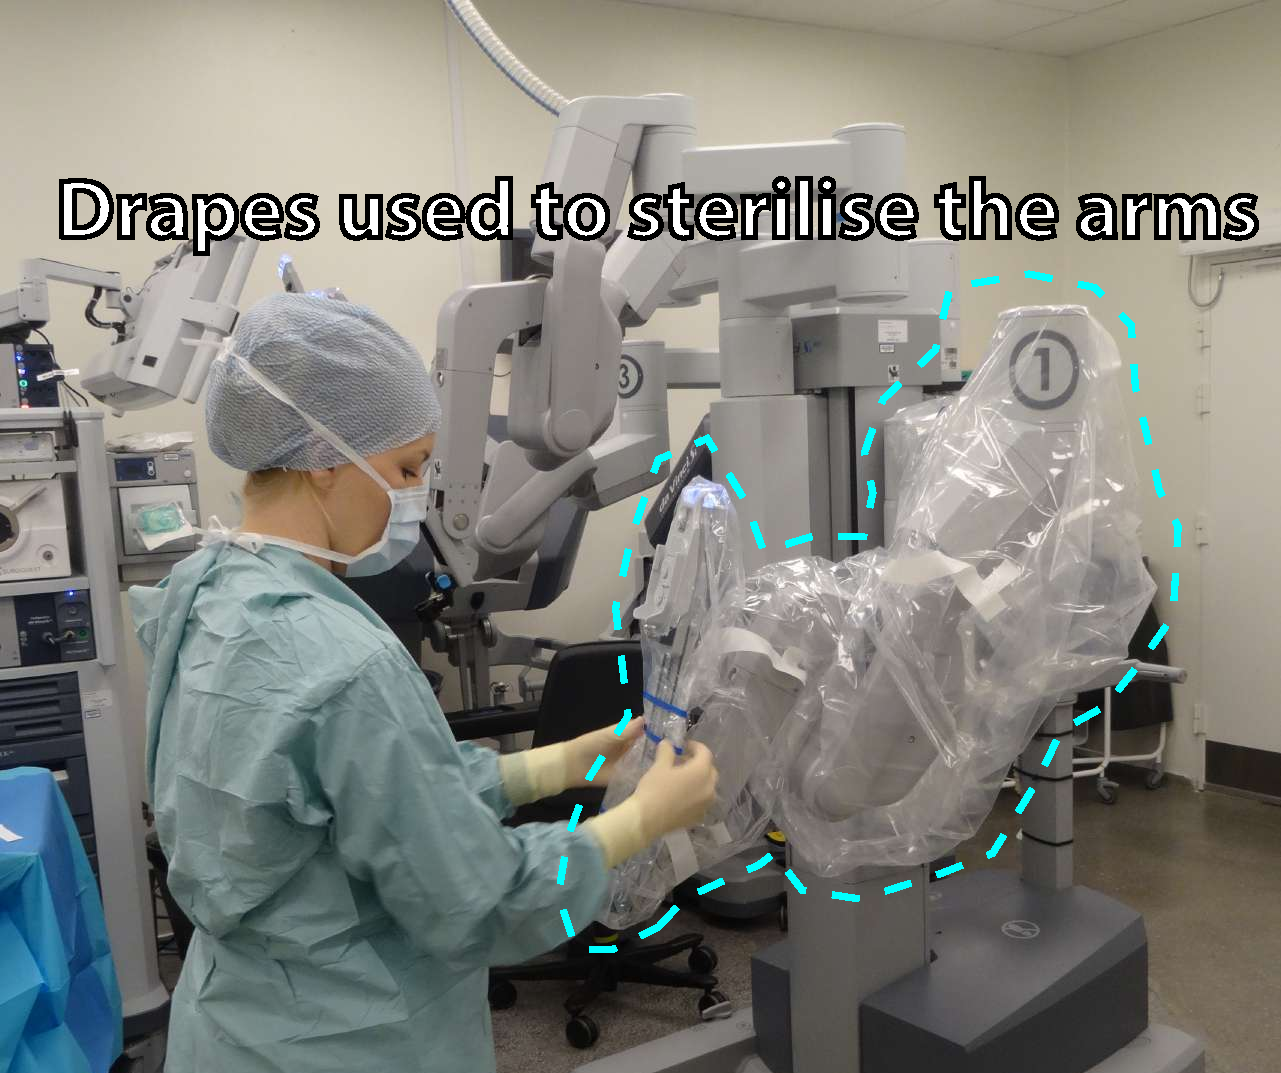
\includegraphics[width=0.6\textwidth]{FieldStudies/figures/drapes.pdf}
	\caption{The drapes used to cover the arms of the robot, sterilising them}
	\label{fig:drapes}
\end{figure} 

\begin{figure}[H]
	\centering
	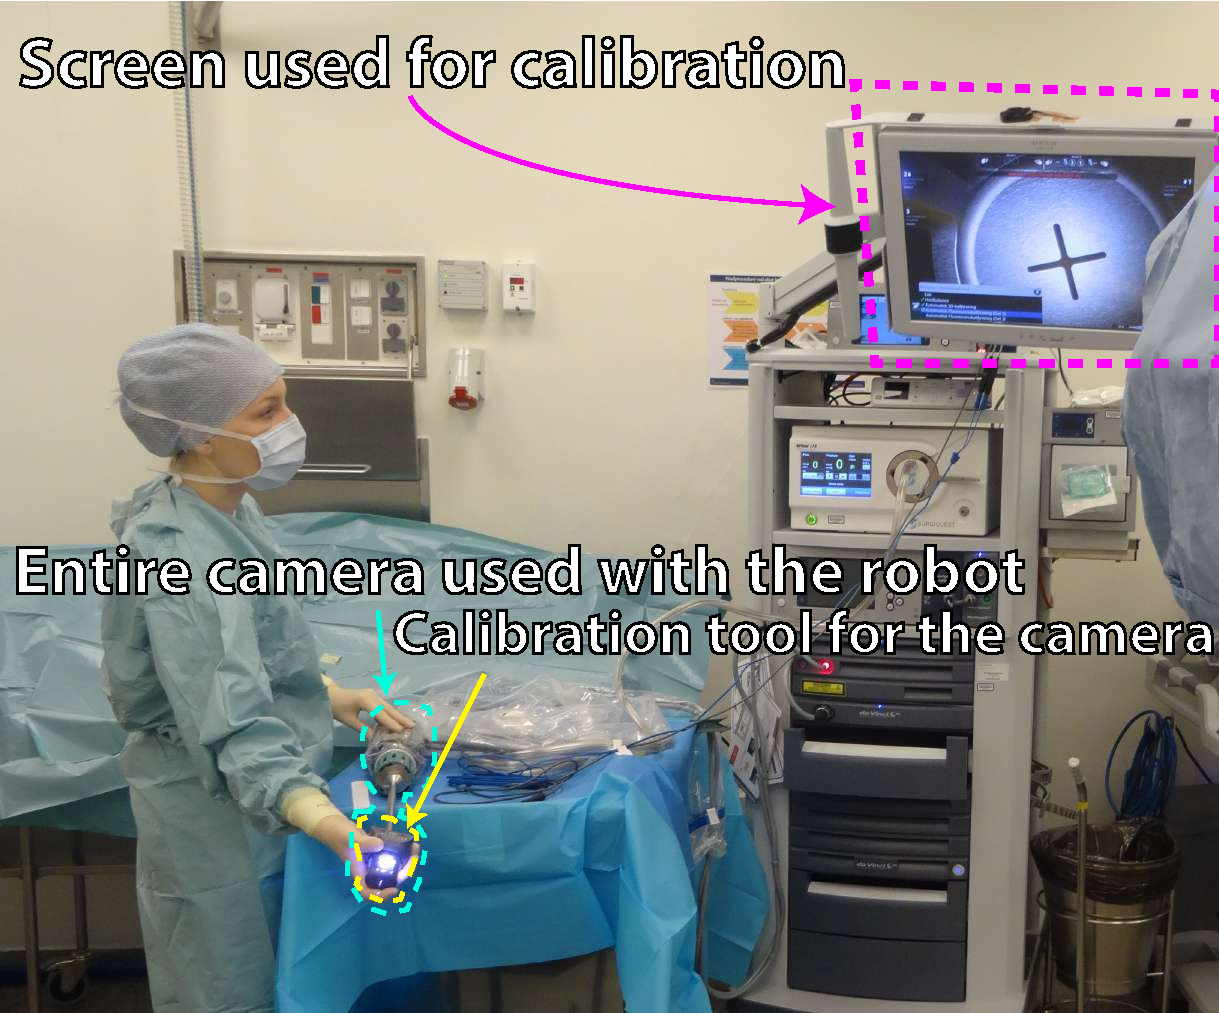
\includegraphics[width=0.6\textwidth]{FieldStudies/figures/camera.pdf}
	\caption{The camera used with the robot and a calibration tool}
	\label{fig:camera}
\end{figure}

\begin{figure}[H]
	\centering
	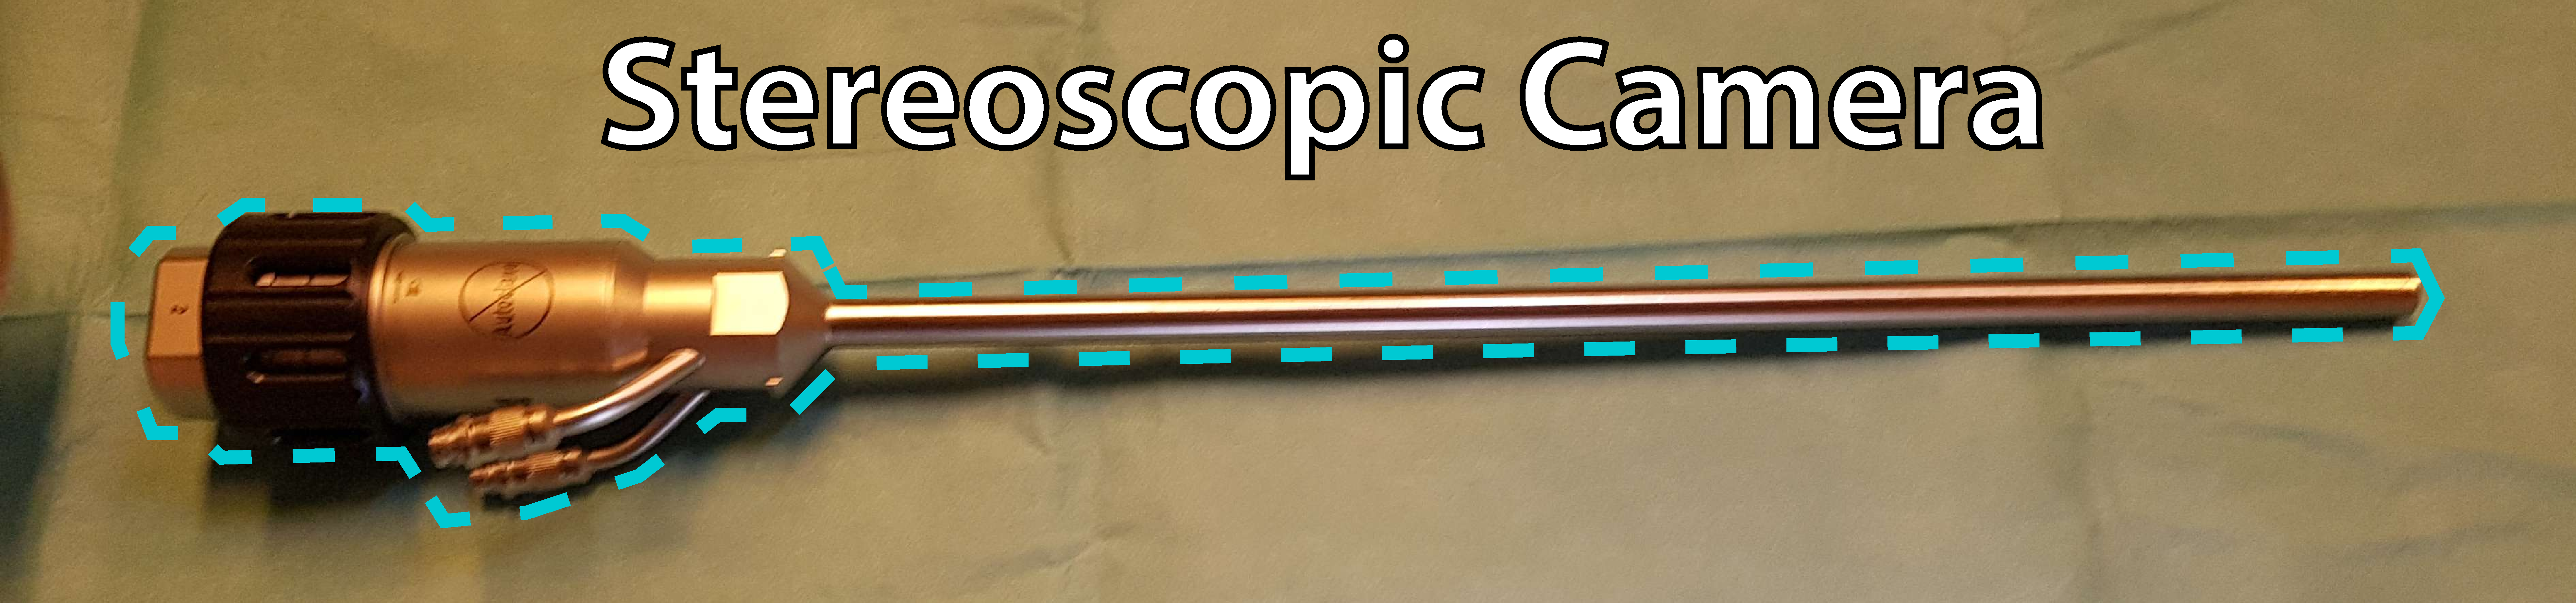
\includegraphics[width=0.6\textwidth]{FieldStudies/figures/camera_close}
	\caption{The endoscopic camera up close}
	\label{fig:cam_close}
\end{figure}

\begin{figure}[H]
	\centering
	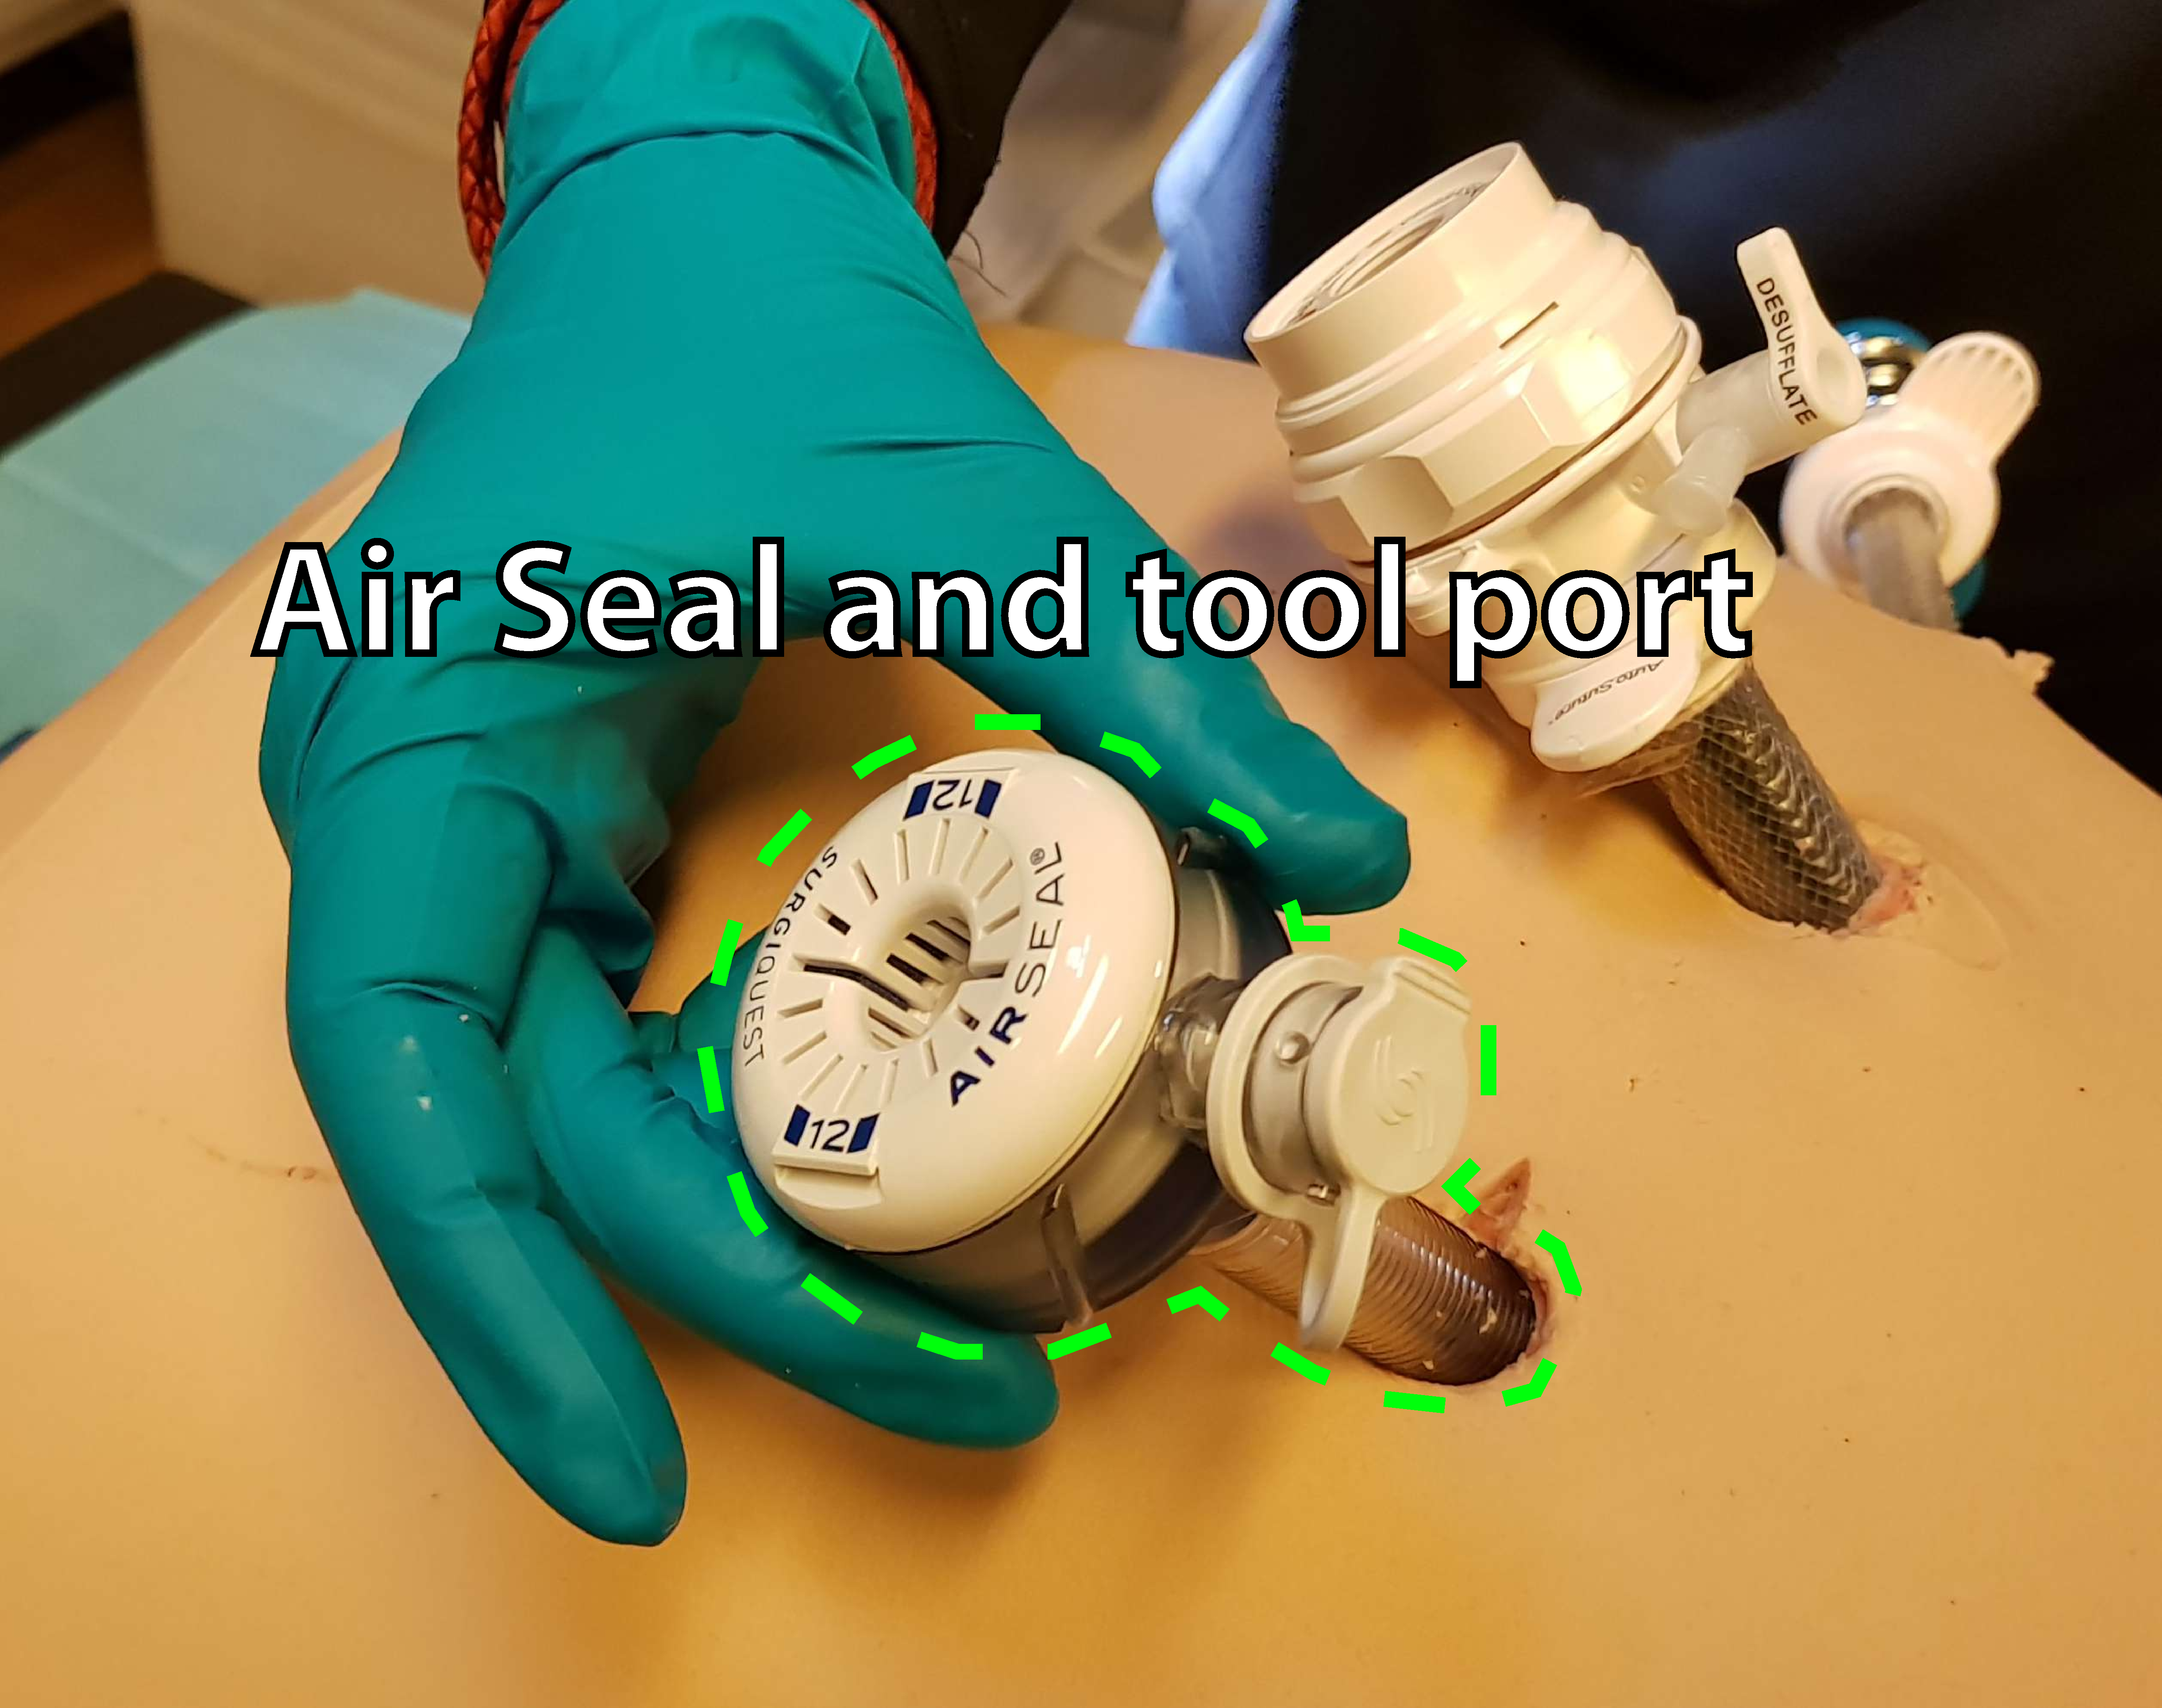
\includegraphics[width=0.6\textwidth]{FieldStudies/figures/port}
	\caption{One of the ports used to insert the tools in the patient}
	\label{fig:port}
\end{figure}

\begin{figure}[H]
	\centering
	
\includegraphics[width=0.6\textwidth]{FieldStudies/figures/tools}
	\caption{The tools used with the robot}
	\label{fig:tools}
\end{figure}


%\subsection*{Evaluation}
%Jane Petersson and Johan Poulsen were both able to test the system. The following interview revealed that the system at present was satisfactory at simulating the scenario, but was not comprehensive enough to warrant implementation with them. They believed the interaction was sufficient, and that trainees didn’t require additional features, however they both stated that several features should be available to the instructors, such as scene change and reset, interacting with procedures and progress, as well as changing the rules during play (for example by introducing emergencies).
%
%One key point throughout the interview was realism. This was brought up many times during the interview, and the consensus was that the closer the simulation was to total realism, both with controls, models, and textures, the more it could replace or improve upon current training standards. This meant that, for example, the robot should have multiple end effectors to allow more realistic movement. The current da Vinci model has three control points and can rotate around itself which the simulated model does not. In addition, the robot itself should be moveable. Introducing tool ports would, together with the improved handling, allow for teaching docking and undocking in VR. Despite all this, draping the robot arms would need to be practiced at real facilities due to the need for accurate tactile feedback.
%
%Johan Poulsen stated that there were limitations, but that systems such as this could be a must-have for the future of RAMIS. He talked about fully integrating the system with current simulators such as RAMIS console and anaesthetic nurse simulators. This could allow full surgery team training. As noted from the context study, Jane Petersson sabotages the robot setup during team training in order to train the nurses’ and doctors’ communication and emergency handling skills. Being able to control even more factors in virtual reality, such as patient fever, would allow for more detailed training of both nurses and surgeons. This concept could also be extended to include scenarios and scenario control. By being able to reset the scene and load a scenario where the setup is an appendectomy would also improve the utility of the system thereby having multiple scenarios to choose from.
%
%Despite its limitations, the current version could be used to introduce medical students to RAMIS if realism was improved. Johan Poulsen also mentioned that, as there was no tactile feedback, the visuals in the scene had to become more realistic as the vision would overcompensate for the lack of tactile feedback. 
%
%Despite the current limitations both experts agreed that the controls of the system were intuitive and that the learning curve was appropriate for their level of expertise with VR. Observations also showed that they both learned to teleport, grab, and interact with the robot fast.


\section*{Conclusion}
The observations and interviews have given an insight as to how both the surgeons and the nurses train and work with the da Vinci Surgical System. Furthermore, critical procedures have been explained by Jane Petersson. These procedures are a must know as failures within these could prove critical or even fatal. The contextual inquiry has been used to determine implementation requirements and key considerations for the expert review. The script for this interview is shown in \autoref{ch:interview_script}.

%The concept of introducing VR training in established RAMIS training sessions seems feasible, however with some caveats. Currently, the system is too basic to warrant implementation at MIUC according to Johan Poulsen, but could serve other purposes such as introducing medical students to RAMIS. Experts stated that the system would require a high level of realism to accurately show the procedure and be useful in RAMIS training.


%\section{Interview Script Including Notes}\label{sec:interview_script}
We firstly introduce Jane and Johan to the simulation. They will get to watch one from the group “play around”, while being explained how the controls work etc. 
The robot will be in un docked position, but the patient is still on the table. The 4 ports, camera and 3 tools are presented on the tool table, they can insert these and “play around”. 
Afterwards they will be able to try the simulation themselves and evaluate the scene.

\subsection{Simulation Feasibility}
\textit{Which aspects of the simulation works well?}
\begin{itemize}
	\item The basic functionality is working well.
	\item The squares which was used to control the robot may need an indication of the orientation
	\item Nice that the instruments could be socketed
	\item The room itself worked well
\end{itemize}

\textit{Which aspects of the simulation does not work well?}
\begin{itemize}
	\item The cart needs to be moved closer to the patient.
	\item The arms didn’t work properly, as they weren’t moving in the same as the real robot did.
	\item The instruments should be able to move instead of just pointing down. 
\end{itemize}

\textit{Is anything crucial missing from the simulation?}
\begin{itemize}
	\item More realism in general. 
	\item You should be able to see the other “players” with each their dedicated roles.
	\item Working together.
	\item Being able to go from the nurse position and docking the robot to sitting at the console and operate the robot. – A full simulation of the surgery.
	\item Even expanding with anaesthetics and information hereof.
	\item Implementing disaster/accidents as well, which you would need to adept to.
\end{itemize}

\textit{Is anything in the simulation redundant/superfluous?}
\begin{itemize}
	\item No
\end{itemize}

\textit{How would you describe the realism of the simulation? How did it affect the experience?}
\begin{itemize}
	\item Nice and spacious.
	\item Needs more realism to be considered a useful simulation
\end{itemize}

\textit{What details did you find missing/lacking in the scene?}
\begin{itemize}
	\item The console is missing from the simulation
	\item Ports in the patient, to give an end goal for the. Maybe attach the arms to the ports and make insertion of the tools in the ports.
	\item When the arms are docked they should still be movable, but around the port socket of course.
\end{itemize}

\subsection{Further Work}
\textit{What is the next step for us to implement?}
\begin{itemize}
	\item 5 ports and making the arms’ endpoints socket to the ports. 
	\item Results of too much force
	\item It is too basic, but the idea has great potential.
	\item Refinement and realism are key points.
\end{itemize}

\textit{What would you use this kind of simulation for? Opportunities, purposes, direction of development.}
\begin{itemize}
	\item As of right now, it may be able to give a basic idea to a completely new user. But it’s not detailed enough. People will not be able to train with this simulation. It has a lot of simulation.
	\item It’s too basic right, but with further development, it can yield enormous possibilities. 
\end{itemize}

\textit{Could it be used for showcasing?}
\begin{itemize}
	\item As before, it should be refined and more realistic, but it is a possibility to use it to showcase what is going on, how the team work together and what is going on.
\end{itemize}

\textit{Do the controls suit your needs? How?}
\begin{itemize}
	\item The two control options are good.
	\item A reset button for a “mentor”/admin/supervisor. 
	\begin{itemize}
		\item A laser pointer which should be visible for everyone. 
		\item Regular controls as well.
	\end{itemize}
	\item Admin controls to switch pre-set scenarios and the different kinds of operations/setups.
\end{itemize}

\textit{Which scenarios are important as well?}
\begin{itemize}
	\item Role designation
\end{itemize}

\textit{What would be nice to have later on?}
\begin{itemize}
	\item A complete simulation of a surgery where you’re able to do everything which is done in real life.
	\item Tactile feedback would be nice – but you use your eyes and compensate as you know the visual signals.
	\begin{itemize}
		\item We could use the vibration in the controllers
	\end{itemize}
	
\end{itemize}